\section{Experimentos e resultados}
    Para a execução dos experimentos, foi utilizado framework PyTorch, para a criação dos modelos, e do ultralytics, para o treinamento com a YOLO.
    
    \subsection{Modelo de detecção}
        Para a realização da detecção, optou-se pelos modelos YOLOv11m e YOLOv12m, treinados utilizando a biblioteca do Ultralytics. O treinamento foi conduzido por 25 épocas, com critério de paciência de cinco épocas. Tanto o otimizador quanto a taxa de aprendizado (\textit{learning rate}) seguiram os valores padrão da função de treinamento do YOLO.

        Após a conclusão do treinamento, os modelos foram avaliados nos dados de teste, e foram calculadas as métricas mAP, precisão, recall e F1-score para as predições. Os resultados obtidos estão apresentados na Tabela \ref{tab:yolo_results}.

        \begin{table}[!htb]
            \centering
            \begin{tabular}{| c | c | c | c | c | c | c | }
                 \hline
                 Modelo & mAP50 & mAP75 & mAP50-95  & Precisão & Revocação & F1 Score\\
                 \hline
                 YOLOv11m & 0.99  &  0.93 &  0.77     &   0.99    &  0.99  &  0.99\\
                 \hline
                 YOLOv12m & 0.99 & 0.94 & 0.77 & 0.99 & 0.99 & 0.99 \\
                 \hline
            \end{tabular}
            \caption{Resultados de teste da YOLO}
            \label{tab:yolo_results}
        \end{table}

        Com tais valores, percebe-se que os modelos identificaram, de forma excepcional, a presença dos eixos nas imagens, possuindo uma baixíssima taxa de falsos-positivo, como observado pela precisão, e uma alta detecção dos objetos, como mostra o recall, resultando em um ótimo valor para o F1-Score.

        No que se refere à localização dos eixos, observou-se que, ao permitir maior flexibilidade, os modelos conseguiram prever suas posições com maior precisão. Esse comportamento é evidenciado pelo resultado do mAP50-95, uma métrica mais rigorosa, que atingiu um valor de 0.77. No entanto, ao considerar uma margem de flexibilidade maior, verificou-se um aumento significativo na qualidade das predições, refletido no mAP75 (0.93 para a YOLOv11 e 0.94 para a YOLOv12) e no excepcional mAP50 (0.99).

        As predições realizadas pelo YOLOv11 podem ser observadas nas figuras \ref{fig:predicao_yolo_1}, \ref{fig:predicao_yolo_2} e \ref{fig:predicao_yolo_3}, sendo valores muito similares para a YOLOv12. Nota-se que o modelo identificou os eixos dos caminhões de forma bastante precisa. Entretanto, a confiança das predições situou-se em torno de 85\%, o que pode ter impactado o resultado do mAP50-95. Dessa forma, levanta-se a hipótese de que métricas ainda melhores poderiam ser alcançadas com anotações mais precisas e consistentes nas imagens de treinamento.

        \begin{figure} [!htb]
            \centering
            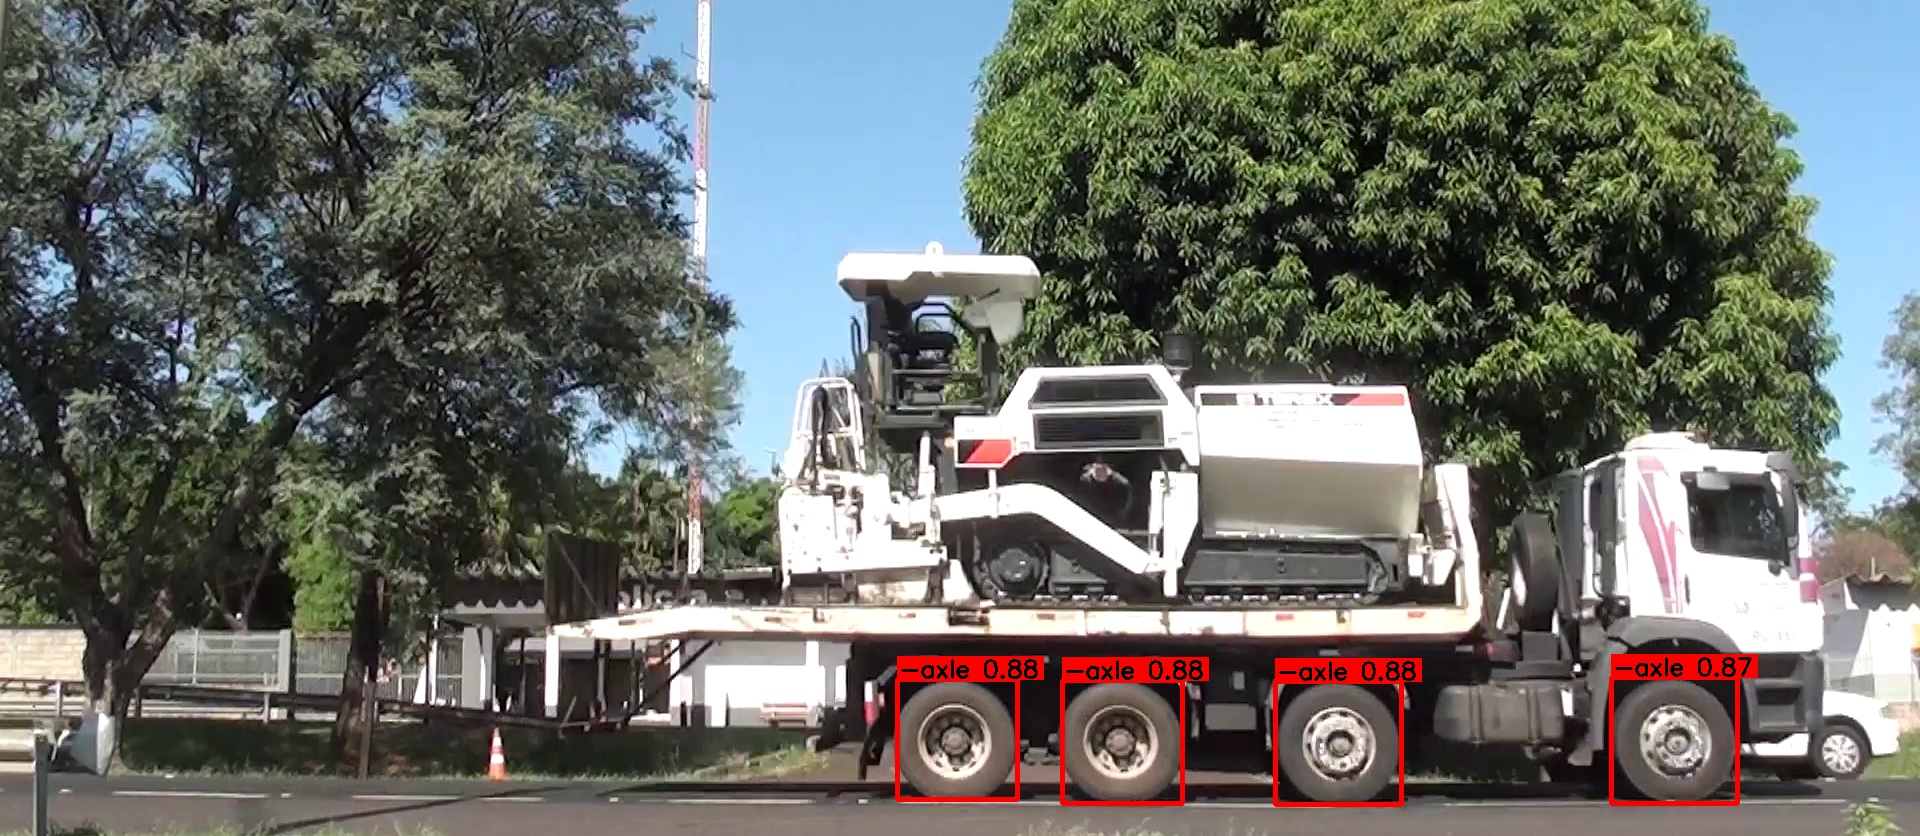
\includegraphics[width=1\linewidth]{Images//yolo_outputs/yolo_output_20170418095402_color-[ROI-1]-94(1).jpg}
            \caption{Predição pelo modelo YOLO com caminhão de quatro eixos}
            \label{fig:predicao_yolo_1}
        \end{figure}

        \begin{figure} [!htb]
            \centering
            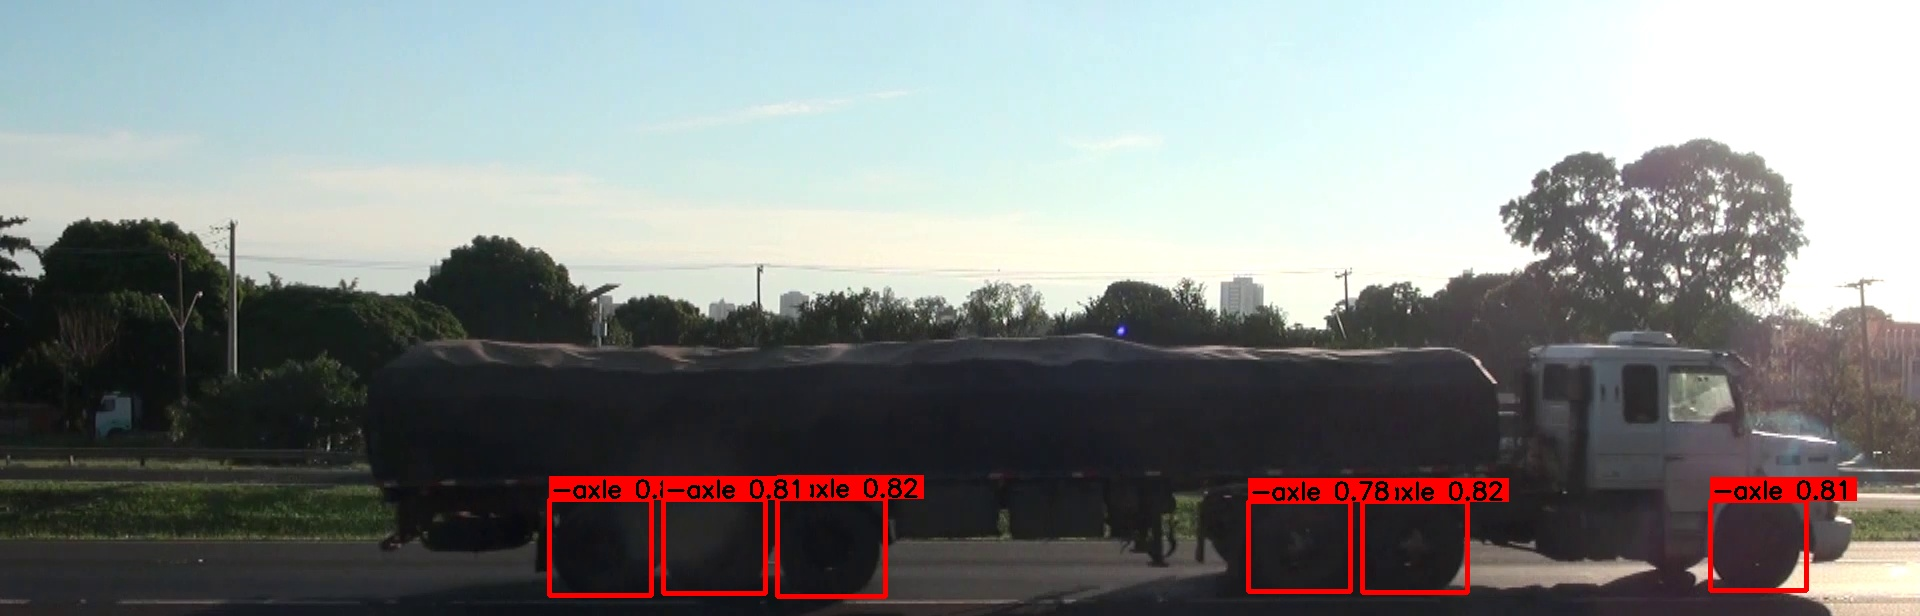
\includegraphics[width=1\linewidth]{Images//yolo_outputs/yolo_output_20170418074140-550_color-[ROI-1]-30.jpg}
            \caption{Predição pelo modelo YOLO com caminhão de seis eixos}
            \label{fig:predicao_yolo_2}
        \end{figure}

        \begin{figure} [!htb]
            \centering
            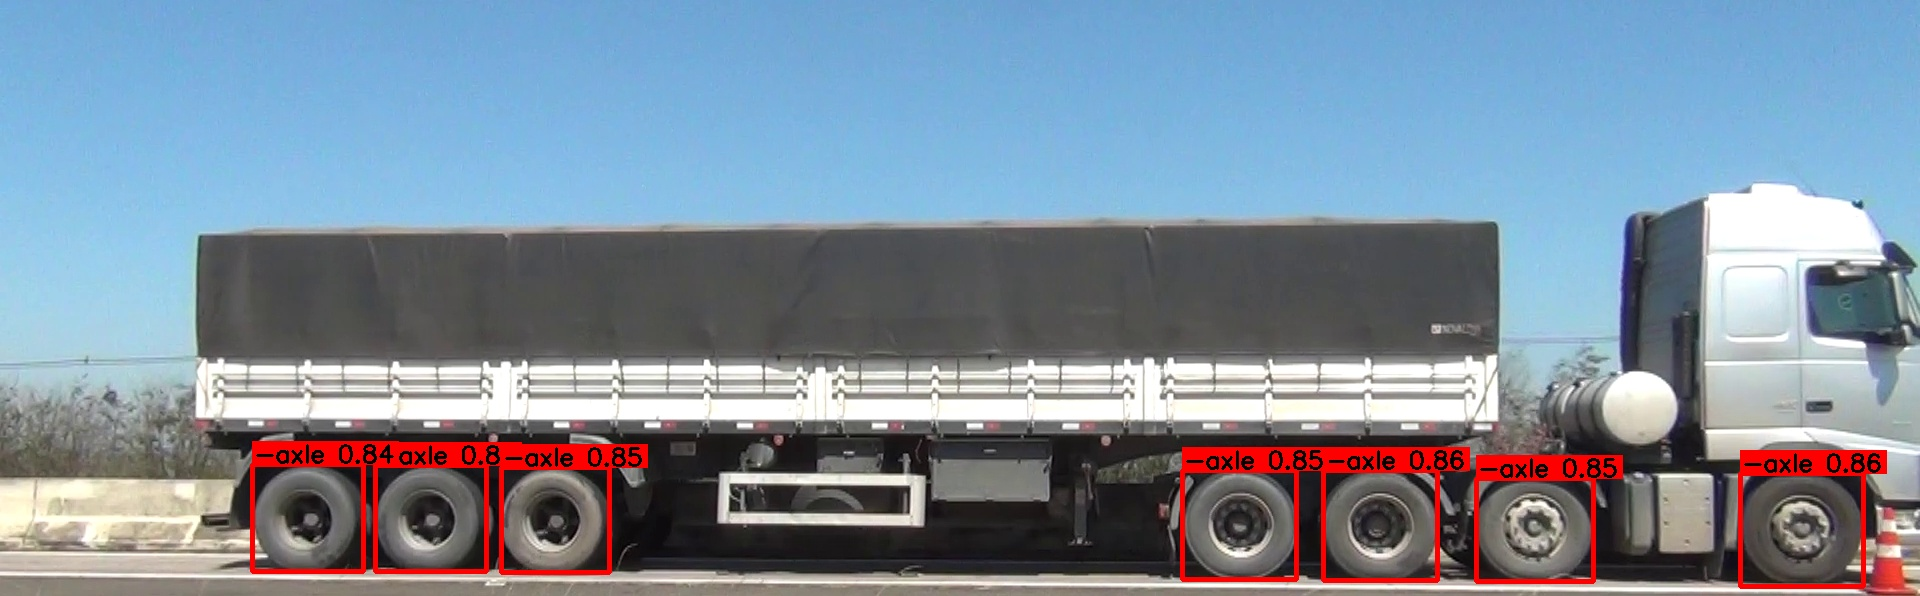
\includegraphics[width=1\linewidth]{Images//yolo_outputs/yolo_output_20160927102749_color-[ROI-1]-1.jpg}
            \caption{Predição pelo modelo YOLO com caminhão de sete eixos}
            \label{fig:predicao_yolo_3}
        \end{figure}
        
    \subsection{Modelos de contagem}
        Para os modelos de regressão que realizam a contagem de eixos, foram analisados dois modelos para transferência de aprendizado, a InceptionV3 (utilizada em \cite{Almutairi2022}) e a ResNet152 (uma versão mais robusta da utilizada em \cite{iluminacao_adversa}), uma vez que mostraram bons desempenhos em tarefas semelhantes envolvendo veículos.

        A estrutura dos modelos é a mesma para ambos e pode ser vista na figura \ref{fig:modelo_base}. A entrada corresponde a uma imagem RGB de 640x640 pixeis, alimentando as redes InceptionV3 e a ResNet, que se conectam a uma camada densa com 512 neurônios e ativação ReLU, seguida de uma camada densa com 256 neurônios, ativação ReLU e BatchNormalization, depois há uma camada densa com 32 neurônios e ativação ReLU, e, por fim, uma camada densa com um neurônio, mas sem ativação.

        \begin{figure}[!htb]
            \centering
            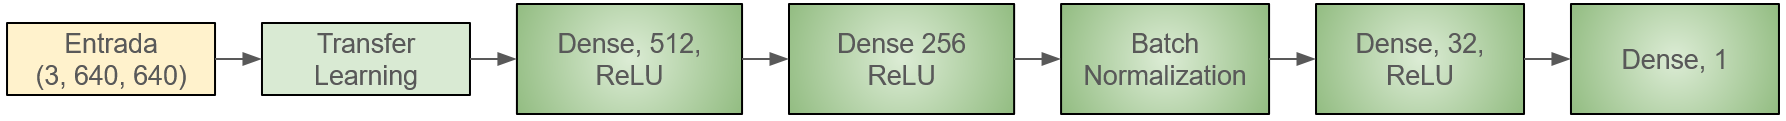
\includegraphics[width=1\linewidth]{Images/modelo.png}
            \caption{Modelo base}
            \label{fig:modelo_base}
        \end{figure}

        Os modelos foram treinados utilizando o otimizador SGD, com \textit{learning rate} de 0.001 e \textit{momentum} de 0.9, tendo como função de erro a Mean Squared Error (MSE). O treinamento poderia ser realizado por até 25 épocas; no entanto, para mitigar o risco de \textit{overfitting}, foi implementado um mecanismo de \textit{Early Stopping} com paciência de três épocas, monitorando o erro de validação como critério de interrupção.
        
        Após o treinamento, os modelos foram avaliados utilizando o conjunto de teste. Para cada imagem, foi realizada uma predição, cujo resultado foi arredondado. A partir desses valores, foram calculadas a precisão, o \textit{recall}, o F1 Score e a acurácia de cada modelo. Além disso, os modelos baseados na YOLO também foram comparados, considerando apenas a quantidade de eixos identificados, sem levar em conta sua localização.
    
        \begin{table}[!htb]
            \begin{tabular}{| c | c | c | c | c | c | c |}
                \hline
                Modelo      & Precision & Recall & F1 Score & Acurácia & Teste loss & MAE Loss \\
                \hline
                ResNet152 & 0.85 & 0.87 & 0.85 & 0.91 & 0.10 & 0.24 \\
                InceptionV3 & 0.88 & 0.85 & 0.86 & 0.92 & 0.12 & 0.22 \\
                YOLOv11m & 0.93 & 0.95 & 0.94 & 0.96 & 0.06 & 0.05    \\
                YOLOv12m & 0.91 & 0.92 & 0.92 & 0.94 & 0.08 & 0.06 \\
                \hline
            \end{tabular}
            \caption{Avaliação dos modelos}
            \label{tab:avaliacao}
        \end{table}

        A tabela \ref{tab:avaliacao} apresenta os resultados obtidos da avaliação dos modelos. Dessa forma, percebe-se que o modelo implementado com a YOLOv11 supera os demais, mesmo que ainda apresentem resultados competitivos, principalmente a InceptionV3 e a YOLOv12. 

        Realizando as predições para as mesmas imagens que geraram as saídas vistas nas figuras \ref{fig:predicao_yolo_1}, \ref{fig:predicao_yolo_2} e \ref{fig:predicao_yolo_3}, obteve-se as predições vistas na tabela \ref{tab:predicao}.        

        \begin{table} [!htb]
            \centering
            \begin{tabular}{| c | c | c | c | c |}
            \hline
            Imagem               & Modelo      & Predição & Arredondamento & Valor real          \\
            \hline
            \multirow{4}{*}{Figura \ref{fig:predicao_yolo_1}} & ResNet      & 6.30     & 6              & \multirow{4}{*}{7}  \\
                                 & InceptionV3 & 5.95     & 6              &                     \\
                                 & YOLOv11m    & 7        & 7              &                     \\
                                 & YOLOv12m    & 7        & 7              &                     \\
            \hline
            \multirow{4}{*}{Figura \ref{fig:predicao_yolo_2}}   & ResNet      & 5.71     & 6              & \multirow{4}{*}{6}  \\
                                 & InceptionV3 & 5.80     & 6              &                     \\
                                 & YOLOv11m    & 6        & 6              &                     \\
                                 & YOLOv12m    & 6        & 6              &                     \\
            \hline
            \multirow{4}{*}{Figura \ref{fig:predicao_yolo_3}}   & ResNet      & 4.01     & 4              & \multirow{4}{*}{4}  \\
                                 & InceptionV3 & 3.76     & 4              &                     \\
                                 & YOLOv11m    & 4        & 4              &                     \\      & YOLOv12m    & 4        & 4              &                     \\                    
            \hline
            \end{tabular}
            \caption{Predição dos modelos}
            \label{tab:predicao}
        \end{table}

        Assim, com tais resultados que corroboram com os dados vistos na tabela \ref{tab:avaliacao}, percebe-se que o uso da YOLOv11 é mais atrativo até mesmo para a tarefa de contagem de eixos. Ademais, o seu custo computacional inferior aos modelos que usam CNN's fazem com que o seu uso seja ainda mais adequado, mesmo no contexto em que, segundo o seu artigo, a YOLOv12 possa ser mais rápida.
            

\section{Conclusão}
    A partir de testes com diferentes arquiteturas e modelos, foi possível identificar uma configuração que se destacou em relação às demais, apresentando alta taxa de acertos e menor custo computacional. Tal modelo é o que foi refinado a partir da YOLOv11m, alcançando um F1 Score de 0.99 na detecção de eixos. No entanto, os valores do mAP50-95 ainda podem ser aprimorados por meio de uma definição mais precisa das \textit{bounding boxes} nas imagens.

    Para trabalhos futuros, seria interessante considerar o uso de imagens capturadas em períodos noturnos, bem como explorar modelos capazes de diferenciar distintos veículos na cena, em vez de agrupá-los como um único objeto. Essa abordagem seria essencial para a implementação de um sistema em tempo real capaz de lidar com múltiplos veículos simultaneamente.